\documentclass{beamer}

% --- Theme and Colors ---
% We'll use a clean, professional theme.
\usetheme{Madrid}
\usecolortheme{beaver} % A nice color scheme
\setbeamerfont{title}{size=\huge}
\setbeamerfont{frametitle}{size=\Large}
\setbeamerfont{section}{size=\Large}
\setbeamerfont{subsection}{size=\normalsize}

% --- Packages ---
\usepackage[utf8]{inputenc}
\usepackage{graphicx}
\usepackage{hyperref}
\usepackage{amsmath}

% --- Presentation Info ---
\title[AI for Cancer Care]{Utilizing Modern Technology for Enhanced Efficiency}
\subtitle{A Strategic Approach to Data and AI in Cancer Care}
\author{}
\date{\today}

% --- Document Starts Here ---
\begin{document}

% --- Title Slide ---
\begin{frame}
    \titlepage
\end{frame}

% --- Slide 2: The Challenge ---
\begin{frame}{The Current Challenge}
    \begin{itemize}
        \item \textbf{Data Fragmentation:} Critical patient data is often scattered across disparate systems and formats.
        \item \textbf{Operational Inefficiencies:} Legacy or manual systems create data silos, impeding workflows.
        \item \textbf{Untapped Potential:} The wealth of patient data is not being leveraged for advanced research or decision-making.
    \end{itemize}
\end{frame}

% --- Slide 3: Our Proposed Approach ---
\begin{frame}{Our Proposed Approach: Leveraging Open-Source}
    \begin{itemize}
        \item \textbf{Core Principle:} Employ a phased, modular technical implementation using established open-source tools.
        \item \textbf{Expert Guidance:} Our role is to provide technical leadership and a clear architectural roadmap.
        \item \textbf{Sustainable Solutions:} Build systems that are not reliant on a single vendor and can be maintained and evolved by the institution.
    \end{itemize}
\end{frame}

% --- Slide 4: Phase 1: Foundational Solutions ---
\begin{frame}{Phase 1: Foundational Solutions}
    \frametitle{Improving Efficiency with a Modern EMR}
    \begin{itemize}
        \item \textbf{Goal:} Centralize patient information to streamline operations and create a digital foundation.
    \item \textbf{Solution:} Implement and customize a robust open-source EMR system, such as OpenMRS.
        \item \textbf{Benefits:}
        \begin{itemize}
            \item Real-time access to patient records.
            \item Improved clinical and administrative workflows.
            \item Immediate efficiency gains for staff.
        \end{itemize}
    \end{itemize}
\end{frame}

% --- Slide 5: Phase 2: Data Ingestion & AI ---
\begin{frame}{Phase 2: Data Ingestion \& Integration}
    \frametitle{Unlocking Insights with a Unified Data Platform}
    \begin{itemize}
        \item \textbf{Goal:} Create a secure and scalable pipeline for multi-modal data.
        \item \textbf{Process:}
        \begin{enumerate}
            \item \textbf{Ingestion:} Securely gather data from various sources (radiology, pathology, genomics).
            \item \textbf{Curation:} Anonymize and clean the data to ensure privacy and quality.
            \item \textbf{Integration:} Combine diverse data modalities into a single, comprehensive view.
        \end{enumerate}
    \end{itemize}
\end{frame}

% --- Slide 6: Phase 3: Downstream AI Tools ---
\begin{frame}{Phase 3: Downstream AI Tools}
    \frametitle{Applying AI for Clinical and Research Impact}
    \begin{itemize}
        \item \textbf{Goal:} Apply machine learning and deep learning models to the integrated data for clinical insights.
        \item \textbf{Examples:}
        \begin{itemize}
            \item \textbf{Computer Vision:} AI-assisted detection and segmentation of tumors in medical images.
            \item \textbf{Natural Language Processing:} Extracting structured insights from clinical notes.
            \item \textbf{Predictive Analytics:} Developing models to forecast patient outcomes and treatment response.
        \end{itemize}
    \end{itemize}
\end{frame}

% --- New Slide for Sustainability ---
\begin{frame}{Creating a Sustainable Future}
    \frametitle{Long-Term Vision: A Dedicated Foundation}
    \begin{itemize}
        \item \textbf{The Challenge:} How to ensure continuous funding for innovation, maintenance, and growth.
        \item \textbf{The Solution:} Establish a dedicated non-profit foundation to support the initiative.
        \item \textbf{Benefits:}
        \begin{itemize}
            \item Secures long-term financial stability.
            \item Attracts sustained philanthropic and CSR support.
            \item Establishes a permanent institution for AI-driven cancer research.
        \end{itemize}
    \end{itemize}
\end{frame}

% --- Architecture Plan Section ---
\begin{frame}{Architecture Plan: System Overview}
    \frametitle{Oncology Data Platform Architecture}
    \begin{center}
        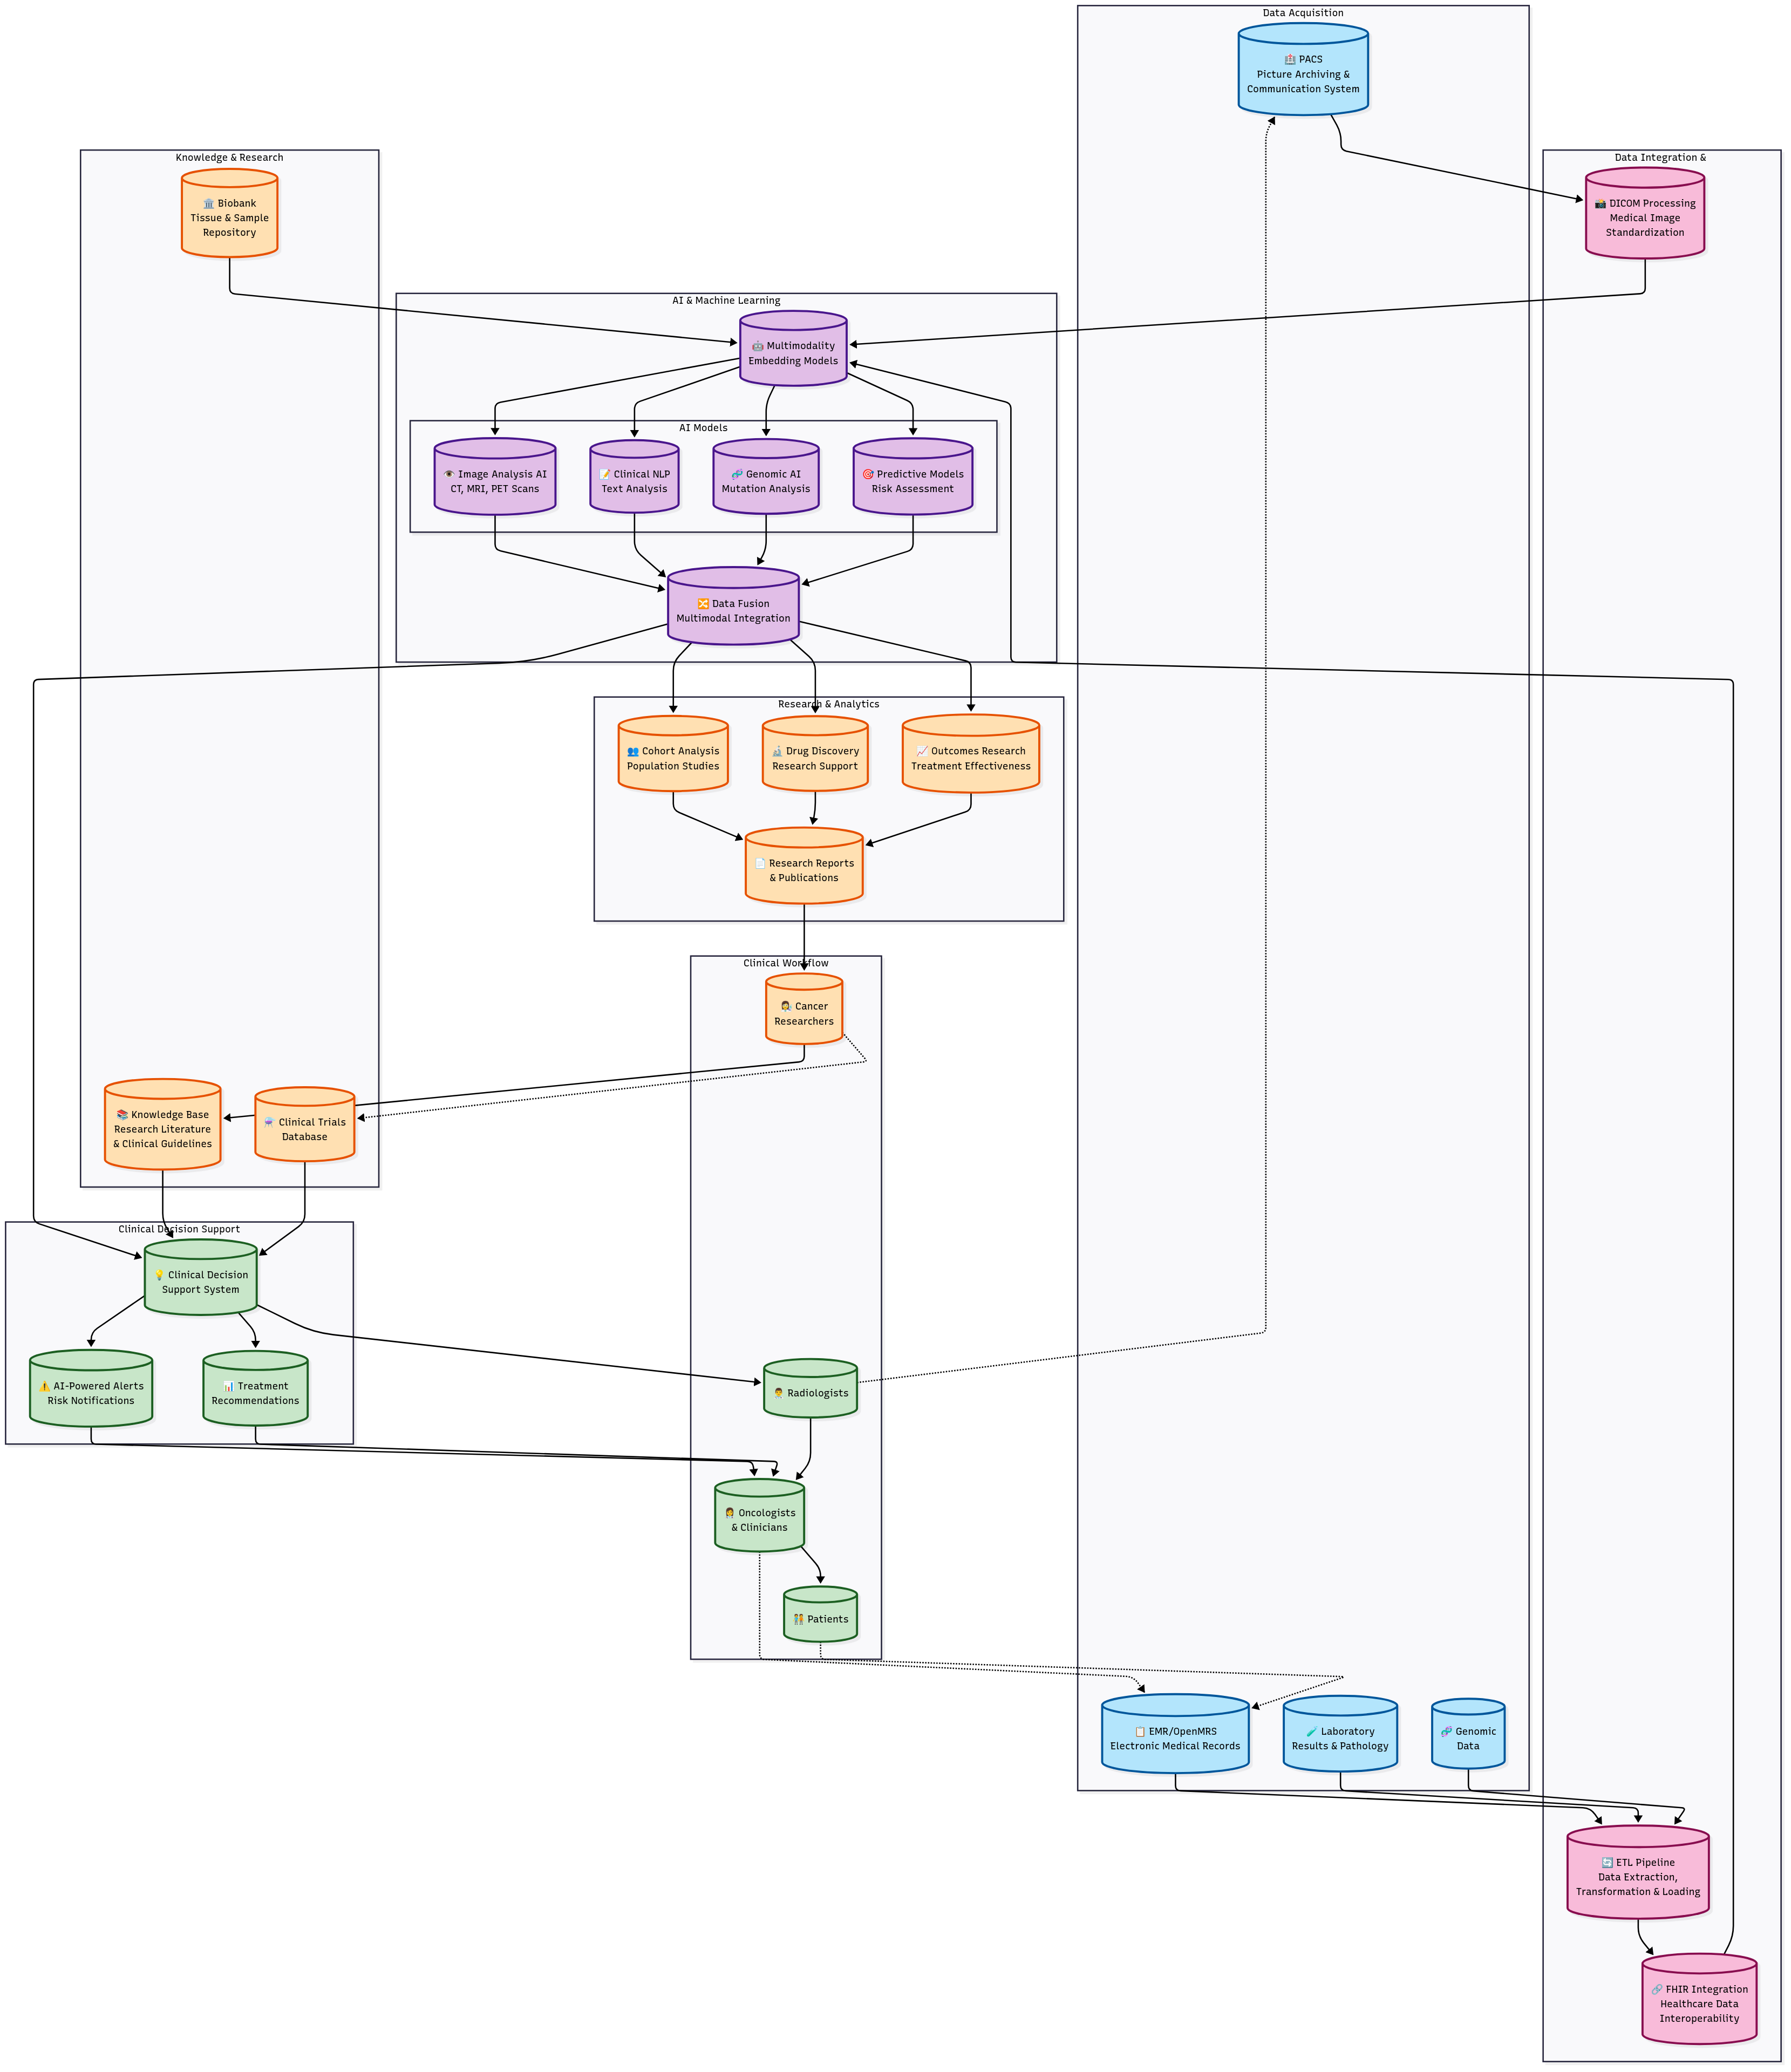
\includegraphics[width=0.5\textwidth]{oncology_platform.png}
    \end{center}
\end{frame}

\begin{frame}{Architecture Plan: Overview}
    \frametitle{AI-Enabled Healthcare System Architecture}
    \begin{itemize}
        \item \textbf{Goal:} Create an integrated ecosystem where PACS, EMR/OpenMRS, and AI work seamlessly together
        \item \textbf{Key Components:}
        \begin{itemize}
            \item Data acquisition layer (PACS, EMR, Laboratory, Genomics)
            \item Integration \& processing middleware (ETL, DICOM, FHIR)
            \item AI/ML analytics engine with multimodality embedding models
            \item Clinical decision support and research analytics
        \end{itemize}
        \item \textbf{Benefits:} Unified data view, AI-powered insights, improved patient outcomes
    \end{itemize}
\end{frame}

\begin{frame}{Architecture Plan: Data Sources}
    \frametitle{Foundation Layer - Data Acquisition}
    \begin{itemize}
        \item \textbf{PACS (Picture Archiving \& Communication System):}
        \begin{itemize}
            \item Stores and manages medical images (CT, MRI, PET scans, X-rays)
            \item Provides DICOM-compliant image distribution
            \item Enables radiologists to access and analyze imaging data
        \end{itemize}
        \item \textbf{EMR/OpenMRS (Electronic Medical Records):}
        \begin{itemize}
            \item Central repository for patient clinical data
            \item Tracks patient history, medications, treatments
            \item Supports clinical workflows and documentation
        \end{itemize}
        \item \textbf{Additional Sources:} Laboratory results, pathology data, genomic information
    \end{itemize}
\end{frame}

\begin{frame}{Architecture Plan: Integration Layer}
    \frametitle{Data Integration \& Processing}
    \begin{itemize}
        \item \textbf{ETL Pipeline:} Data extraction, transformation, and loading from multiple sources
        \item \textbf{DICOM Processing:} Medical image standardization and metadata extraction
        \item \textbf{FHIR Integration:} Healthcare data interoperability standard
        \begin{itemize}
            \item Fast Healthcare Interoperability Resources
            \item Enables different healthcare systems to communicate
            \item Uses modern web standards (REST APIs, JSON, XML)
            \item Organizes data into standardized resources (Patient, Observation, etc.)
        \end{itemize}
        \item \textbf{Result:} Clean, standardized data ready for AI analysis
    \end{itemize}
\end{frame}

\begin{frame}{Architecture Plan: AI/ML Engine}
    \frametitle{Multimodality AI \& Machine Learning}
    \begin{itemize}
        \item \textbf{Multimodality Embedding Models:}
        \begin{itemize}
            \item Process multiple data types simultaneously
            \item Combine imaging, text, genomic, and clinical data
            \item Create unified representations for comprehensive analysis
        \end{itemize}
        \item \textbf{Specialized AI Models:}
        \begin{itemize}
            \item \textbf{Image Analysis AI:} CT, MRI, PET scan interpretation
            \item \textbf{Clinical NLP:} Text analysis of medical records
            \item \textbf{Genomic AI:} Mutation and biomarker analysis
            \item \textbf{Predictive Models:} Risk assessment and outcome prediction
        \end{itemize}
        \item \textbf{Data Fusion:} Multimodal integration for holistic insights
    \end{itemize}
\end{frame}

\begin{frame}{Architecture Plan: Clinical Impact}
    \frametitle{Clinical Decision Support \& Research}
    \begin{itemize}
        \item \textbf{Clinical Decision Support System:}
        \begin{itemize}
            \item AI-powered alerts and risk notifications
            \item Evidence-based treatment recommendations
            \item Real-time integration with clinical workflows
        \end{itemize}
        \item \textbf{Research \& Analytics:}
        \begin{itemize}
            \item Population health studies and cohort analysis
            \item Drug discovery and clinical trial optimization
            \item Treatment outcomes research
            \item Knowledge discovery from integrated healthcare data
        \end{itemize}
        \item \textbf{Knowledge Integration:} Research literature, clinical guidelines, biobanks
    \end{itemize}
\end{frame}

\begin{frame}{Architecture Plan: Implementation Benefits}
    \frametitle{Transformative AI Integration}
    \begin{itemize}
        \item \textbf{Early Detection:} AI analyzes imaging patterns for early cancer detection
        \item \textbf{Personalized Treatment:} Combines genomic and clinical data for tailored therapies
        \item \textbf{Risk Stratification:} Predictive models assess patient risk factors
        \item \textbf{Research Acceleration:} Automated analysis of large datasets for research insights
        \item \textbf{Clinical Decision Support:} Real-time recommendations based on evidence and patient data
        \item \textbf{Scalability:} Modular architecture allows for future expansion and integration
    \end{itemize}
\end{frame}

% --- Slide 7: Next Steps ---
\begin{frame}{Immediate Actions}
    \begin{itemize}
        \item \textbf{Phase 1 Kick-off:} Begin a discovery and planning phase to identify the most suitable pilot project for an EMR implementation.
        \item \textbf{Form a Working Group:} Establish a small technical committee with institute staff to assess existing infrastructure.
        \item \textbf{Assess Resources:} Identify internal and external resources that can be leveraged to support the initiative.
        \item \textbf{Discuss Long-Term Funding:} Schedule a follow-up conversation to explore sustainable funding strategies.
    \end{itemize}
\end{frame}

\end{document}
